\chapter{Introduction}
\label{chap:introduction}

\section{Motivation}
The last few decades have seen the most pronounced technology evolution in history, in many different areas and markets: from smartphones to robotics, from cars to medicine, etc. One of the pillars upon which all these advancements have been made possible is the Internet, or more generally the entire set of networking technologies that allow software to communicate. 


The process towards interconnected devices saw a big leap forward in the early 1960s with the first research into packet switching as an alternative to the old circuit switching. But it is 1982 the year of standardization for TCP/IP protocol suite, which permitted the expansion of interconnected networks  [wiki]. The Internet grew rapidly, passing from a few tens of million users in the 1990s to almost 3 billions users in 2014 [\href{http://www.internetlivestats.com/internet-users}{ref}]. Even more astonishing is the number of networked devices and connections globally, around 14 billion in 2014 [\href{http://www.cisco.com/c/en/us/solutions/service-provider/visual-networking-index-vni/index.html#~complete-forecast}{ref}]

\begin{figure}[!htb]
\centering
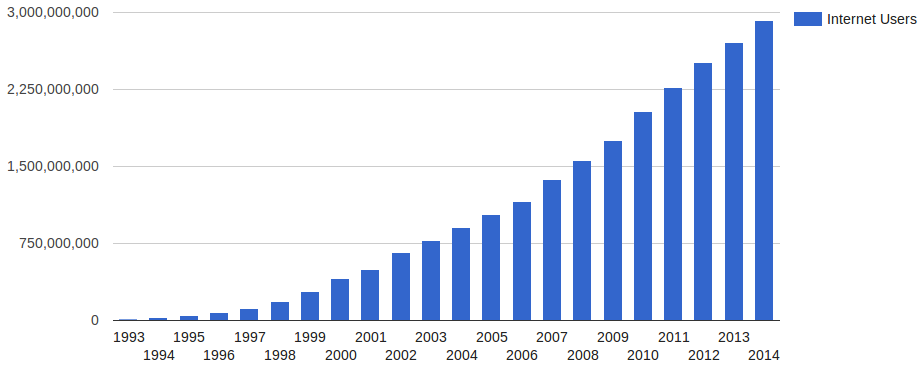
\includegraphics[width=\textwidth]{images/internet_growth}
\caption{The expansion of the Internet}
\label{fig:networkscenario}
\end{figure}

"Networks" is a very generic term. In the IT context it can refer to any set of nodes communicating over a certain protocol. The most widespread protocol for networking communication is the above-mentioned TCP/IP protocol, that is used in the vast majority of services like the World Wide Web, email, file transfer (for example FTP), remote system access, etc. It is also often used as a communication protocol in private networks and datacenters. 
The reason for its wide adoption is not because there aren't good alternatives: TCP/IP is not to most performing protocol in every network environment, but it is fairly simple and it introduces a relatively low complexity in the overall architecture, still guaranteeing all the basic connection requirements. Back in the 1980s, TCP/IP was the simpler way for applications to use most networks, thus quickly becoming a de-facto standard [\href{http://www.computerworld.com/article/2593612/networking/tcp-ip.html}{ref}]. 
During its life, the TCP/IP protocol suite have seen many updates and additional components to reach the desired levels of network congestion, traffic load balancing, handling of unpredictable behaviors, security, user-experience and so on. Such requirements became more and more strict with the uncontrollable expansion of the Internet. Albeit, after all these years the fundamental aspects of the TCP design design haven't been changed at all, mainly for retro-compatibility purposes. This inevitably causes some aspects of the protocol to look very limited in the current networking reality. A striking example is the scarcity of available IPv4 addresses: when TCP was designed in the 1970s, a 32 bits number reserved for addressing all hosts in the Internet seemed to be a very high number. Nevertheless, due to a misuse of address allocation policies and, mainly, due to the unexpected increase in the number of connected devices, the original IPv4 addresses available run out quickly, forcing the introduction of the lengthy 126bit bits address format, known as IPv6. Unfortunately, modifying the original TCP implementation to make use of the new address turned out to be a remarkably complicated procedure overall: to maintain retro-compatibility, IPv6 portion of TCP is implemented as a separate network stack component, and even if nowadays the majority of the systems are IPv6-compatible, it took 20 years to reach the current percentage of overall adoption: 10\% [\href{http://www.google.com/intl/en/ipv6/statistics.html#tab=ipv6-adoption&tab=ipv6-adoption}{ref}].

\vspace{5mm}
When the TCP protocol was first developed in the 1970s, it was certainly difficult to predict the rate of growth of the networks all around the globe, not only in terms of the number of nodes involved, but also in terms of the quantity and type of the transmitted data, the increasing need of low latency for new streaming applications, the advancement in the hardware adopted to carry the data and the computing power of the interconnected devices. Today we can count billions of interconnected devices, and we have just started the era of the IoT (Internet of Things) which aims at giving communication capabilities to virtually every object commonly used in our daily life.
As a result of this process, the networks of today are becoming more intricate and devices often use multiple interfaces to stay connected. Even common appliances like smartphones provide both cellular connectivity and Wi-Fi modules; laptops have at least Wi-Fi capabilities plus an Ethernet port. The argumentation is much more complex in the back-end infrastructures' scenario, where we can find datacenters counting thousands of interconnected nodes and content-delivery servers that are capable of handling a huge number of network interfaces simultaneously.
The implications of this new reality include the possibility of establishing multiple paths to transmit data between pairs of hosts, since they are now often equipped with multiple network interfaces, each with an active IP address. Back in 1970s TCP was designed to create a virtual connection between exactly two IP addresses and two port values, with almost no flexibility or dynamism in address/port addition and/or removal. In the multipath scenario typical of the infrastructures of today, to old point-to-point single-path connection provided by TCP looks quite limiting. This led to various projects aiming at exploiting the multipath concept, and MPTCP is one of them.

\subsection{Benefits of Multipathing}
Multipathing provides hosts with a resource pooling concept applied to networking access. Resource pooling allows dynamism and flexibility in requesting and handling resources and it has been a positive trend in many services and architectures, like CDNs, P2P networks, cloud computing, etc. The very concept of packet-switching is based on a resource pooling technique, where circuit utilization is not using isolated channels but the traffic in a circuit can make use of the spared capacity of other circuits [\href{https://www.cl.cam.ac.uk/~as2330/docs/multipath-survey.pdf}{ref}].
In the multipath context, "resource pooling" might assume slightly different meaning according to the specific implementation and the layer it operates on in the OSI architecture (more on this later). Nevertheless, a general set of benefits can be defined for adopting multipathing-aware technology. Such set is presented in the following list, from the point of view of MPTCP (which operates at the Transport Layer):
\begin{itemize}
  \item Combining MPTCP multipath and multi-homing, it is possible to achieve higher throughput by exploiting multiple simultaneous connections to transfer different portions of the same piece of data. For example, a typical smartphone could use its cellular module and its Wi-Fi module simultaneously in downloading a file from a remote server, despite them having two different IP addresses.
  \item It is possible to introduce failure handover for the connection with no special mechanism at Network or Link Layer. If one of the interfaces goes down or the flow of data gets interrupted for any reason, data transfer can seamlessly continue through other interfaces;
  \item By assigning different priorities to the various interfaces, it would be possible to better handle data consumption (useful in case of a limited-capacity data-plan); for example, consider the case of a file download on a smartphone via 4G connectivity: it would be reasonable to switch the whole data transfer to the Wi-Fi interface if that becomes available in the middle of the download, starting from the point left by the cellular connection and without the need to restart the session;
  \item Providing multipath awareness to current network stacks could improve load balancing and exploitation of the network resources in datacenters; this is a valuable aspect, considering that the network performance in data centers is usually the bottleneck for the latency of the overall system. A similar concept applies for load balancing in ISPs network backbone.
\end{itemize}

\subsection{Multipathing Solutions}
\vspace{5mm}
MPTCP aims at achieving all the benefits mentioned in the previous paragraph. Before MPTCP, other proposals have been elaborated to achieve multipath benefits by introducing new technologies at the Link Layer, Network Layer and even Transport Layer (the same layer on which TCP operates). Even at the Application Layer developers can create custom protocols on top of TCP to achieve benefits similar to those that would come "naturally" by exploiting multipath natively at the lower layers. 
For example, most modern browsers open many TCP connection simultaneously to download the various elements of a Web-Page to improve user experience. Another example could be Skype and similar VOIP programs, which try to automatically reconnect hosts in case of problems with minimum impact on the user experience. Albeit all the solutions at the Application Layer are just clever workarounds on top of regular TCP and they fall only marginally in our argumentation regarding multipath.

The following list gives a general overview of the most important solutions other than MPTCP:
\begin{itemize}
  \item At Link Layer there are link aggregation techniques to aggregate the capacities of different interfaces to the same switch [add a ref]. There are different modes to achieve resource pooling through link aggregation, but the basic concept is to setup multiple interfaces with the same IP address (and usually the same MAC address) so that the link aggregation is transparent to the higher-level applications and various algorithms can be used to redistribute the data packets to the various links. In order for this to work, proper configuration is needed at the host and at the next-hop switch. Despite being a common solution in ISPs' inner networks and datacenters to improve throughput and achieve higher network-access, end-users cannot directly take advantage of this technology.


  \item At the Network Layer there exist multiple solutions to better exploit multipathing, most notably Mobile IP and Shim6. They both provide hot-handover capabilities with no interruption of the higher-level services, with some limitations. Mobile IP requires extensive support by the underlying infrastructure and Shim6 is an IPv6 only solution. More importantly, there is a fundamental problem in introducing resource pooling at the Network Layer: TCP operates at the Transport Layer but it is closely related to the Network Layer because it statefully inspects various properties of the underlying network paths to provide performance optimizations; transparent modifications at the Network Layer would cause consistent TCP malfunctioning.


  \item At the Transport Layer the most notable experiment in multipath exploitation prior to MPTCP is the Stream Control Transmission Protocol (SCTP). Such protocol is, in many ways, similar to MPTCP: the first version of SCTP provided fail-over capabilities by exploiting different interfaces, and successive versions introduced multi-streaming capabilities to increase throughput via different interfaces. The major problem with SCTP is that it was thought to be an alternative enhanced version of TCP, and the two protocol are indeed incompatible with each other. This means that a wide adoption of SCTP would require to upgrade all the middleboxes to be SCTP aware, in order not to discard unrecognized packets. Moreover, all the applications would need to be upgraded to explicitly use the new protocol to communicate. The vast global networking scenario of today, mainly based on TCP, makes these requirement virtually impossible to meet, and today SCTP remains a technology of very limited adoption.
\end{itemize}



\vspace{5mm}
All these previous solutions didn't get widespread adoption. Link Layers and Network Layers solutions require extensive modifications in the underlying network configurations in order to achieve the desired results; introducing a new multipath-aware protocol at the Transport Layer requires to change all the applications in order for them to communicate over the new protocol, thus allowing this solution in very limited scenarios; workarounds at the Application Layer, despite being quite effective, are far from the purpose of MPTCP.

Multipath TCP (MPTCP) is an ongoing project managed by the Internet Engineering Task Force (IETF), whose specifications have been published as Experimental standard in January 2013 [ref RFC 6824]; since then, the protocol has seen a lot of interest in the Internet community and many implementations quickly became available for the most common platforms. 
MPTCP primary goal is to automatically introduce the multipath benefits to current infrastructures and devices, with the minimum possible effort from users, developers, network maintainers. Engineers decided that the best way to achieve all these requirements was to still make use of TCP as fundamental block, exploiting its extensible TCP Options field to introduce all the custom options needed to handle multipath subflows: the entire protocol design works by adding MPTCP custom options into regular TCP packets, so that MPTCP-aware systems can process such options; if a system that is not MPTCP-aware receives a MPTCP connection-request, it would simply discard the MPTCP options and threat such packet as a plain TCP connection-request. All the subflows connecting the various interfaces in a MPTCP session would look like normal TCP connections to the lower infrastructure. Retro-compatibility is achieved with most of the current systems. For what regards applications, they don't need to be changed either since MPTCP would be inserted into the network stack at the operating system level, it would automatically split the data coming from the Application Layer and send it through different subflows, according to the number of available endpoints at the connected hosts.

\vspace{5mm}
MPTCP not only aims at providing all the benefits of multipath, but it is also designed to require the minimum possible effort in large-scale deployment. For these reasons, the new protocol got a lot of attention in the Internet community in the last few years, and many consider MPTCP as a valuable step forward for the whole global network currently relying on TCP.
The final goal of MPTCP is to replace the majority of the current TCP implementations, which is a very delicate process in which all the current TCP standards in terms of robustness and security have to be maintained, if not improved. This paper is an evaluation of the security aspects of MPTCP, with an analysis of current threats and vulnerabilities affecting the protocol.

\section{Problem Statement}
MPTCP is a big effort from the IETF working group to unlock multipath networking capabilities worldwide, with many subtle implications for current infrastructures. Hence the importance of evaluating the current security status of MPTCP, both by inspecting its implications on external middleboxes and security equipment and by analyzing internal design flaws that might allow attacks to the MPTCP sessions. The main focus of this paper is on the latter case. The main vulnerability currently known for the protocol, related to the ADD\_ADDR component, is tested and studied; the solution for it is implemented and evaluated. In the process, actual patches for the Linux kernel implementation of the protocol have been developed to fix the vulnerability. 


A comprehensive list of all the objective for the thesis follows:
\begin{itemize}
    \item Studying the security implications of adopting MPTCP on current infrastructures; 
    \item Listing the known vulnerabilities affecting the current version of the protocol; 
    \item Studying the ADD\_ADDR vulnerability of the protocol;
    \item Evaluating the possible solutions for the ADD\_ADDR vulnerability; 
    \item Assessing the best solution for the ADD\_ADDR vulnerability and developing it for the Linux kernel implementation of MPTCP;
    \item Developing effective and powerful simulation scenarios in order to test MPTCP (and possibly other networking protocols);
    \item Contributing to the upstreaming of MPTCP into the Linux kernel by developing patches and contributing to official RFC documentation.
\end{itemize}

\section{Methodology}
The thesis work has been carried out at the Intel office in Lund, Sweden. The process took 6 months in total, with a main focus on testing and developing. The entire work has been closely followed by major stakeholders in the MPTCP community, located in Sweden, Romania and the United States. Such cooperation involved patch reviewing and weekly meetings.


The work flow started with an overall study of MPTCP and how it interacts with the most common middleboxes. The next step was a more focused evaluation of the current threats for the protocol by using as reference the document RFC 7430. Within the document, only one vulnerability is considered a blocking issue in the advancement of MPTCP standardization, known as the ADD\_ADDR vulnerability. The document also proposes a change in the protocol design that fixes the problem, and with such reference the actual development part of the work started.


At first, it was necessary to sync with the development status by interacting with the official MPTCP mailing list for developers [\href{https://listes-2.sipr.ucl.ac.be/sympa}{ref}]; this allowed to make sure that the ADD\_ADDR solution proposed in RFC 7430 was indeed the preferred one and that nobody started developing a patch for it already.
Before starting to work on the fix, a first stage of the work involved a deeper analysis of the ADD\_ADDR vulnerability. A connection hijacking has been executed by exploiting such vulnerability in a testing environment. This allowed to better validated the criticality of the problem and it was a useful experiment to get acquainted with MPTCP. Moreover, it was a good way to setup a proper testing environment that was indeed used during the whole patch-development process that followed.


After having reproduced the attack there was an analysis of the MPTCP modules within the Linux kernel in order to understand how the protocol implementation works inside the TCP stack. The development work that followed involved side features that came out to be necessary for a proper functioning, including some final testing.